% **************************************************************** %
%                          Document Class
% **************************************************************** %
% Class of the document: KOMA Script Report
%   Options: 12 points font, A4 paper, bibliography in ToC
\documentclass[
	draft,
	a4paper,
	11pt,
	bibliography=totoc,
	headsepline=true,
	footnotes=multiple,
	chapterprefix=true,
	captions=tableheading,
	origlongtable,
	listof=totoc
]{scrreprt}

% **************************************************************** %
%                  User Defined Variables (commands)
% **************************************************************** %
\makeatletter % **** **** **** **** **** **** MAKEATLETTER

% thesis stuff
\newcommand{\thesisTitle}{Sustainable futures of mobility}
\newcommand{\thesisSubtitle}{Transition narratives for policy design and assessment tools}
\newcommand{\authorName}{David}
\newcommand{\authorLastnames}{Martínez Rodríguez}
\newcommand{\authorFullName}{\authorName~\authorLastnames}
\newcommand{\authorEmail}{davidmr@kth.se}
\newcommand{\authorAffiliation}{Sustainable Technology MSc Student, KTH}
\newcommand{\thesisCourseCode}{AL227X}
\newcommand{\supervisorName}{Rajib}
\newcommand{\supervisorLastname}{Sinha}
\newcommand{\supervisorFullName}{Rajib Sinha}
\newcommand{\department}{Industrial Ecology Division, SEED Department}
\newcommand{\departmentFull}{Industrial Ecology Division, SEED Department, ABE School, KTH}
\newcommand{\academicTerm}{Spring 2017}

% format
\newcommand{\acronymsTOCTitle}{List of Abbreviations}
\newcommand{\glossariesTOCTitle}{Glossary}
\newcommand{\TOCTitle}{Table of Contents}
\newcommand{\TOCLinkColour}{DeepSkyBlue4!50!black}

\makeatother % **** **** **** **** **** **** MAKEATOTHER

% **************************************************************** %
%                            Packages
% **************************************************************** %
%\usepackage[top=1in,bottom=1.25in,left=1.25in,right=1.25in]{geometry}								% Custom margins (comment out if not needed)
\usepackage[english]{babel}	% Language settings
\usepackage{etoolbox}
\usepackage{titlesec}
\usepackage{lmodern} % Use Latin Modern font
\usepackage[nointegrals]{wasysym}
\usepackage{microtype} % Enhanced typesetting (better reading)
\usepackage[final]{graphicx}	% Enhanced graphics processing
\usepackage{url}
\usepackage[table,hyperref,x11names,svgnames]{xcolor}	% Allows coloring tables
\usepackage[section]{placeins} % Ensure float elems. inside their section
\usepackage{booktabs}	% Beautiful, professional tables
\usepackage{longtable}
\usepackage{adjustbox} % Boxing capabilities for images and text
\usepackage{multirow}	% Enables tabular cells spanning multiple rows
\usepackage{array} % Enables custom table column defintions
\usepackage[toc,page]{appendix}	% Appendices title customisation
\usepackage{enumitem}	% Customized enumerations and itemizes
\usepackage[version=3]{mhchem} % Allows inclusion of chemical formulas and eq.
\usepackage{amssymb}
\usepackage{siunitx} % SI units standard
\usepackage[textwidth=\marginparwidth,colorinlistoftodos,obeyDraft]{todonotes}
\usepackage{authblk} % Allows authors with affiliations
\usepackage{lastpage}	% Allows referencing the last page
\usepackage[style=british]{csquotes} % Allows block quotations
\usepackage{multicol} % Multicolumn environment
\usepackage[font=small,labelfont=bf]{caption}
\usepackage{pdflscape} % Rotate pages (for wide pages)
\usepackage{subcaption}
\usepackage{nameref}	% Allows references by name ("Section 5" vs "Conclusions")
\usepackage{lipsum} % Lorem ipsum
\usepackage[framemethod=TikZ]{mdframed} % Info boxes
\usepackage[
backend=biber,
natbib=true,
bibstyle=authoryear,
citestyle=authoryear,
sorting=nyt,
block=space,
hyperref=true,
dashed=false
]{biblatex}
\usepackage{hyperref}
\hypersetup{
final,
unicode=true,
pdftitle={\thesisTitle},
pdfauthor={\authorFullName},
pdfpagemode={UseOutlines},
pdfstartview={FitV},
bookmarks=true,
bookmarksopen=true,
bookmarksopenlevel=0,
bookmarksnumbered=true,
breaklinks=true, % to have links breaking among lines
hypertexnames=true,
plainpages=false,
hidelinks=false,
colorlinks=true,
citecolor=DeepSkyBlue4,
filecolor=black,
linkcolor=DeepSkyBlue4, %DeepSkyBlue4!50!black,
urlcolor=DeepSkyBlue4,
anchorcolor=DeepSkyBlue4
}
\usepackage[
acronym,
toc,
nopostdot,
hyperfirst=false
]{glossaries} % Acronyms lists

% **************************************************************** %
%                        Command definitions
% **************************************************************** %
\makeatletter % **** **** **** **** **** **** MAKEATLETTER
% useful cross referencing commands
\newcommand{\fref}[1]{Figure~\ref{#1}}
\newcommand{\tref}[1]{Table~\ref{#1}}
\newcommand{\eref}[1]{Equation~\ref{#1}}
\newcommand{\cref}[1]{Chapter~\ref{#1}}
\newcommand{\sref}[1]{Section~\ref{#1}}
\newcommand{\ssref}[1]{Subsection~\ref{#1}}
\newcommand{\aref}[1]{Appendix~\ref{#1}}
\newcommand{\alref}[1]{Algorithm~\ref{#1}}
\newcommand{\procref}[1]{Procedure~\ref{#1}}

% document parts
\newcommand{\frontmatter}{%
	\cleardoublepage
	\pagenumbering{roman}
	\pagestyle{plain}}
\newcommand{\mainmatter}{%
	\cleardoublepage
	\pagenumbering{arabic}
	\pagestyle{headings}}
\newcommand{\backmatter}{%
	\cleardoublepage
	\pagestyle{plain}}

% author "and" for title page
\renewcommand\Authands{ and }

% the norm of vectors
\newcommand{\norm}[1]{\lvert #1 \rvert}

% todo's
\renewcommand{\todo}[2][]{%
	\@bsphack\@todo[fancyline,#1]{#2}\@esphack\ignorespaces}%
\newcommand{\todocite}[1]{\todo[size=\footnotesize,color=green!40]{#1}}
\newcommand{\todonote}[1]{\todo[size=\footnotesize]{#1}}
\newcommand{\todoparagraph}[1]{%
	\todo[color=yellow!40,bordercolor=yellow!40,inline]{#1}}
\newcommand{\todowarning}[1]{%
	\todo[color=red!40,bordercolor=red,inline]{#1}}
\newcommand{\todocomment}[1]{%
	\todo[color=teal!40,bordercolor=teal,inline]{#1}}

\makeatother % **** **** **** **** **** **** MAKEATOTHER

% **************************************************************** %
%                          New environments
% **************************************************************** %
% checklist environment
\newenvironment{checklist}{%
  \begin{list}{}{}% whatever you want the list to be
  \let\olditem\item
  \renewcommand\item{\olditem[$\Box$] }
  \newcommand\checkeditem{\olditem[$\CheckedBox$] }
}{%
  \end{list}
}

\newenvironment{enumeratealpha}{%
	\begin{enumerate}[label=(\alph*)]
}{%
	\end{enumerate}
}

%% Infobox style
% Setting box counter
\newcounter{infobox}[chapter]
\renewcommand{\theinfobox}{\thechapter.\arabic{infobox}}
% The environment
\newenvironment{infobox}[1][]{%
    \refstepcounter{infobox}
    \begin{mdframed}[%
        frametitle={Box \theinfobox\ #1},
        skipabove=\baselineskip plus 2pt minus 1pt,
        skipbelow=\baselineskip plus 2pt minus 1pt,
        leftmargin=12pt,
        rightmargin=12pt,
        frametitleaboveskip=7pt,
        frametitlebelowskip=7pt,
        linewidth=0.5pt,
        linecolor=black,
        frametitlerule=true,
        frametitlebackgroundcolor=white,
        backgroundcolor=white,
        roundcorner=0pt,
    ]%
    \sffamily
}{%
    \end{mdframed}
}

% **************************************************************** %
%                               Format
% **************************************************************** %
% Koma Script font modifications
\setkomafont{author}{\small}
\setkomafont{date}{\scshape}
\setkomafont{caption}{\normalsize} % needed because longtables with smaller text
  % have to be "surrounded" by \footnotesize groups, thus reducing caption sizes
\renewcommand*{\bibfont}{\small}
\renewcommand{\captionformat}{~}

% Row spacing for booktabs tables
\renewcommand{\arraystretch}{1.1}

% Formatting for paragraphs (indentation and space after par.)
\setlength{\parskip}{0.5\baselineskip}%
\setlength{\parindent}{0pt}%
%\setlength{\textfloatsep}{8pt plus 1.0pt minus 2.0pt}
%\setlength{\floatsep}{5.0pt plus 1.0pt minus 1.0pt}

% Column separation for multicols environment
\setlength{\columnsep}{2em}

% Enumerations and lists separation
%\setlist{itemsep=-0.25\parskip}

% SI units range separator (en-dash)
\sisetup{range-phrase=--}
% New SI units
\DeclareSIUnit{\tex}{tex}
\DeclareSIUnit{\yr}{yr}
\DeclareSIUnit{\person}{person}

% Reduce space after sections
\titlespacing{\section}{0pt}{\parskip}{-0.5\parskip}
\titlespacing{\subsection}{0pt}{\parskip}{-0.5\parskip}
\titlespacing{\subsubsection}{0pt}{\parskip}{-0.5\parskip}

% Configuration of the blockquotes paragraphs
\SetBlockThreshold{1} % all blockquotes of 1 or more lines are treated as blocks

% **************************************************************** %
%                   Glossaries and References
% **************************************************************** %

% Glossaries (acronyms) files
\makeglossaries % BEFORE the inclusion of glossaries

% Redefine glossaries so that the first entry is hyperlinked but not
% subsequent appearances
\renewcommand{\glsentryfmt}{%
  \ifglsused{\glslabel}
    {\glsgenentryfmt}% entry has been used.
    {\glshyperlink[\glsgenentryfmt]{\glslabel}}% entry hasn't been used
}

% Load glossary file (acronyms, etc.)
\newacronym{IPCC}{IPCC}{International Panel on Climate Change}
\newacronym{SSP}{SSP}{Shared Socio-economic Pathway}
\newacronym{SSP1-MOB}{SSP1-MOB}{Extended Mobility SSP Scenario}
\newacronym{IAM}{IAM}{Integrated Assessment Model}
\newacronym{SD}{SD}{Sustainable Development}
\newacronym{PT}{PT}{public transport}
%\newacronym{<label>}{<abbrv>}{<full>}

% References files (BibTeX's)
\addbibresource{references.bib}

% **************************************************************** %
%                            Title page
% **************************************************************** %
\title{\vspace{1cm}\thesisTitle}
\subtitle{\thesisSubtitle\vspace{8cm}}

\author{\authorFullName (\footnotesize\texttt{\authorEmail})}
\affil{\authorAffiliation}

	% Hijacked \date command to add course information
\date{
	\todowarning{!!! Turn this into the generated KTH cover and back pages !!!}
	\textsc{\thesisCourseCode~MSc Thesis}\\
  	\textsc{\departmentFull}\\
	\textsc{\academicTerm}\\[0.5cm]
	\today
}

% **************************************************************** %
%                             Document
% **************************************************************** %
\begin{document}
% Title page
\maketitle
\thispagestyle{empty}

% Front matter: abstract, table of contents, acknowledgements...
%   !they are all Roman numbered!
\frontmatter
%%%%% Abstract page %%%%
\cleardoublepage % Clear the previous page
\phantomsection % Create Hyperref anchor
\addcontentsline{toc}{section}{Abstract} % Add the abstract to the Table of Contents

\section*{Abstract} % Abstract section, unnumbered ("*")
Today the world is consuming almost \SI{70000}{\mega\tonne} of apparel every year, this accounts for $2\%$ of the world’s GDP and presents a large threat to the environment \parencite{icac2013}. One way to reduce the environmental impact is to change to another type of fabric than the traditional ones. This report is investigating if Swedish viscose could be that type of fabric, it is labelled as a natural product since it is produced from wood pulp. The LCA is conducted for two of T-shirts made from Swedish viscose and Asian cotton. The functional unit is a cotton or viscose T-shirt of \SI{200}{\g} during its whole life cycle, including the disposal phase, used in Sweden during 2 years, washed once every two weeks (for a total of 52 wash cycles). The system boundary for this study is cradle-to-grave. The impact categories that are assessed for the study are \textit{freshwater eutrophication}, \textit{terrestrial ecotoxicity} and \textit{water depletion}. The LCA study shows that the viscose T-shirt has the lowest overall impact compared to the cotton T-shirt. A sensitivity analysis is conducted by remove the tumble dryer in the use phase. The lack of LCI data for making a T-shirt with viscose fabric could reduce the credibility of the results, future LCA studies are needed with data from the production phases of a viscose T-shirt.

\cleardoublepage % Clear the page for other sections (front matter or main matter)

\tableofcontents % Content Index
\listoffigures
\listoftables
\printglossary[type=\acronymtype,title={\acronymsTOCTitle}]
\todototoc %should be placed right before the \listoftodos command
{\footnotesize \listoftodos}

% Main matter: the actual content of the report
\mainmatter
\chapter{Introduction}
\label{c:introduction}

This thesis report is an investigation of sustainable mobility futures. It is a theoretical exploration of how policy can deliver the necessary efforts and guidelines for a successful a transition to a sustainable mobility system. \emph{What} is understood for ``sustainable'' and \emph{how} the transition is to be managed and envisioned are the main foci of the document. Special emphasis is put on the \emph{cultures} of mobility and on achieving the widest \emph{system perspective} as possible. This being said, a clarification must be made already regarding a limitation in the scope of this study: the concept of ``mobility'' that is used throughout the thesis is bound to personal travel, i.e., not freight transport.

Overall, the report structure adheres the IMRAD+C paradigm, with the present \nameref{c:introduction} chapter, followed by the \nameref{c:methods}, \nameref{c:results}, \nameref{c:discussion} and, finally, the \nameref{c:conclusion}. With regards to this introductory chapter, \sref{s:intro:unsustainable-mobility} presents an overview of the pressing issues of the current mobility system. A state of the art review with respect to policy approaches and design tools is given in \sref{s:intro:state-of-art}. To conclude the chapter, \sref{s:intro:aim-objectives} states the aims and objectives that motivate the rest of this research.

\section{Unsustainable mobility}
\label{s:intro:unsustainable-mobility}
Several issues of the current mobility system make it qualify as unsustainable. Direct downstream impacts, e.g. greenhouse gas emissions, are the most directly perceivable hazards, but it is their combination with global future trends that increases the significance of mobility impacts on sustainability. Issues such as population growth \parencite{un-desa2015_WorldPopulationProspects,kc2017_humancoreshared}, peak oil \parencite{kerr2011_Peakoilproduction}, expected impacts from climate change and growing economies in Asia, South-America and Africa, all highlight the acceleration and exponential expansion of the negative effects that high mobility poses to the environment, the economy and to human health and social systems.

Transport related airborne pollution is one of the main causes of respiratory diseases and associated increase in morbidity in densely populated areas~\parencite{vimercati2011_Trafficrelatedair,who2006_Airqualityguidelines}. Ambient air pollution is estimated to cause 4.4 million premature deaths around the globe~\parencite{forouzanfar2016_Globalregionalnational} and the link from air pollution to both severe health problems and high traffic volumes is well known and thoroughly researched~\parencite{who2006_Airqualityguidelines}: \ce{NO_x} emissions that lead to increases in \ce{PM_{2.5}} particulate and ozone concentrations are directly linked to diesel combustion engines, in heavy duty but also light duty vehicles \parencite{anenberg2017_Impactsmitigationexcess}. The fact that regulations and emission limits are in place within the automotive industry has not alleviated the problem, due to ever-growing automobile use and because of the industry efforts to deceive such regulations, avoiding costly research and development investments, as is the case of the recent ``dieselgate'' scandal \parencite{guardian2017_Volkswagenrevealsrecord}.

The current unsustainable mobility system not only causes respiratory health issues, but also congestion, accidents, noise pollution, infrastructure degradation and, finally, it is one of the sectors that most contribute to climate change \parencite{korzhenevych2014_UpdateHandbookExternal}. Congestion is, for example, the cause of massive costs in terms of reduced productivity, increased energy and fuel consumption, higher accident risk and its subsequent economic impacts which, for instance, are estimated at 4.2\% of Beijing's 2010 GDP\footnote{Gross Domestic Product} ~\parencite{li-zeng2012_SocialCostTraffic}. Road-related accidents alone (cars, buses and other vehicles aggregated) cause vehicle losses and damages and, most importantly, death rates that exceed 1.2 million worldwide per year or \num{28077} in the European Union (EU) in 2015 \parencite{who2017_GlobalHealthObservatory}. Safety in rail and aviation is much higher (especially per person kilometre travelled) than in roads, but they still take away 993 lives in rail-related accidents and 155 in aviation (EU data, 2015) \parencite{eurostat2017_StatisticsExplainedRailway,eurostat2017_EurostatOnlineDatabase}.

The transport sector is responsible for 27.8\% of the global final energy consumption (2014 data), with over 95\% of this energy coming from fossil sources (oil, primarily, but natural gas and coal too) \parencite{iea2017_Statisticswebportal}. \textcite{chapman2007_Transportclimatechange} already estimated that 26\% of the total world's \ce{CO_2} emissions were borne in the transport sector, of which 65\% are originated in road transport. Given the enormous pressure that climate change puts on the resilience of modern societies \parencite{ipcc2014_ClimateChange2014} and the current undertaking to tackle this global challenge --- take, for example, the recent Paris Agreement Framework Convention on Climate Change \parencite{clemencon2016_TwoSidesParis} ---, transport (mobility) is one of the sectors that must be thoroughly examined, revised and challenged to deliver urgent greenhouse gas emissions mitigation.

\subsection{Automobility at the core}
\label{ss:intro:automobility-at-core}
Automobility, as a personal mobility solution, has brought about many positive consequences, from the individuals point of view. However, its exponential growth and reliance on fossil fuels and massive infrastructures to work deem it as a global threat to the environment and, at a more local scale, to the quality of life of the very same individuals that make use of this transport mode. Given that automobility accounts for almost 36\% of the travel demand (in person kilometres per year) \parencite{vuuren2017_Energylanduse}, and that 65\% of \ce{CO_2} emissions from all travel modes are attributed to road transport \parencite{chapman2007_Transportclimatechange}, it is logical to state that automobility is, indeed, a major player in the sustainable mobility discussion. Therefore, this thesis will place a good deal of emphasis on this particular mode. The study scope encompasses the relation between this regime and public transport, or between automobility and urban planning, for example --- limiting the scope of this research to the automobile system would certainly not be sufficient to address the broad concept of sustainable mobility.

%\subsection{The need for a transition}
%\label{ss:intro:need-for-transition}
%
%\todoparagraph{Introduce the necessity of a transition (because impacts and expected growth in those due to population/affluence growth, etc. etc.)}
%
%There is therefore, at the environmental, social and economic levels, a societal need for a transition away from the current dominant regime of automobility. A new sustainable mobility paradigm is to emerge if we are truly committed to a sustainable future. How this paradigm may look like is not clear and needs further investigation from a future studies perspective.

\section{State of the art}
\label{s:intro:state-of-art}
%To address all the aforementioned issues, policy packages or simultaneous enforcing of different policies are needed, because of the complexity involved in effectively reducing transportation impacts~\parencite[ch. 3, p. 45]{garciasierra2014_Travelbehaviourenvironmental}. Regulation cannot, however, be designed without evaluating the caused impacts, at any level, in the short and long term -- too many resources and possible negative outcomes would be at stake. \textit{Policy assessment} from the systems thinking perspective is, therefore, a key issue to develop, due to the difficulty of dealing with entire systems, their internal dynamics and the emergent systemic behaviour patterns, such as feedback loops, rebound effects and hidden causalities. In this regard, the field of \textit{system dynamics} can help capture such structures and cause-effect chains \parencite{hjorth2006_Navigatingtowardssustainable}. The holistic nature of system dynamics models can help achieving an integrated assessment framework for urban mobility policies, by delivering information on a set of several indicators, at the environmental, social and economic levels.
%
%Finally, there is another perspective to be considered in the thesis. Policy development in the field of transportation has been mainly focused on two paths, according to \textcite{koehler2009_transitionsmodelsustainable}, to increase the sustainability of the system: (a) efficiency increasing measures, by means of incentives for technological enhancements (e.g. better engines or fuel mixes) and more stringent pollution limits and (b) behavioural change management, i.e., measures aimed at modal shift -- encouraging people to shift from private cars to public transport, for example. Both approaches, albeit successful to some extent, have not delivered the expected results so far, due to the high inertia and stabilization mechanisms inherent to the current dominant regime for transportation: internal combustion engines cars-based mobility \parencite{geels2012_AutomobilityTransitionSocio}. However, a third way is possible, when it comes to policy design for sustainable mobility: \textit{transition management oriented policy} (TMOP).
%
%The approach of TMOP entails adopting a longer term thinking mindset (usually one or several generations), multi-level and multi-domain thinking, maintaining support for a large set of solutions and with a focus in system \textit{innovation} alongside system \textit{improvements} \parencite{rotmans2001_Moreevolutionthan}. Moreover, flexibility in the objectives of policies is encouraged, as well as a more qualitative perspective to policy goals. All these characteristics configure a policy design mindset that could be the key to unlock a true game change in urban mobility, by drifting the focus from quantitative, efficiency measures to a transition and innovation vision, where something more than technological progress is harnessed to achieve a sustainable transport system in the future.

Historically\footnote{The historical time-frame considered in the thesis goes back to the beginning of the 20th century.}, in the ``advanced'' economies of Europe and North-America, personal mobility issues such as congestion and accessibility\footnote{Accessibility is meant as the capacity of reaching (travelling) a destination from ``any'' other given point in a territory.} have been addressed through the development of infrastructure, through increased incentives for automobility and, to some extend, travel demand management \parencite{lyons2012_VisionsFutureNeed}. Policy solutions for environmental social impacts of automobility have also been focused on technological improvement and, to some extent, modal shift\footnote{Modal shift refers to changes in the shares of travel modes (reducing car use in favour or biking, for example)} \parencite{koehler2009_transitionsmodelsustainable}.

However effective these policies were in the past --- the paradigm of ``predict-and-provide'' for infrastructure development (to address congestion) has already been dismissed in the UK, being regarded as non-efficient and even counter-productive \parencite{goodwin2012_ProvidingRoadCapacity} ---, it is clear that they are not so nowadays. Faced with pressing global trends like population growth and the fact that emergent economies in Asia and South-America are also embracing automobility as the paradigm of personal mobility, pressure keeps building on the natural and social environments. A new policy approach is needed; one that is capable of transforming the mobility system into a more sustainable one. Some efforts have been taken to fill this gap, through policy assessment tools like, for example, sustainability indicator frameworks \parencite{castillo2010_ELASTICmethodological,haghshenas2012_Urbansustainabletransportation,litman2007_DevelopingIndicatorsComprehensive,shiau2013_Developingindicatorsystem}.

Despite the best of the intentions behind them, policy assessment tools such as indicators have not performed as expected. Most indicator frameworks are not used as they should, i.e., for their instrumental and operational roles. Instead, policy makers just use them as another source of information, because they claim that ``sets of numbers'' do not convey the necessary insights for policy design or formulation \parencite{gudmundsson2013_SomeuseLittleinfluence}. One of the main drawbacks of indicators is that they are focused on \emph{impact} assessment. Policy design should not be focused on a responsive approach -- a proactive, driver-based approach is the key to a sustainable mobility transition. There is a need to model and conceptualize the ``engine'' of the mobility system and, then, find leverage points for effective policy design. Other traditional policy assessment tools, such as Integrated Assessment Models, are much broader and do evaluate the drivers of the transport sector, but fail to capture the social dimension of the system (they tend to be focused on economic variables and trends such as fuel prices) \parencite{creutzig2015_EvolvingNarrativesLow}. The hypothesis held in this study is that traditional policy assessment tools lack either the systems perspective necessary to avoid policy resistance\footnote{\emph{Policy resistance} refers to unexpected responses of a system to a certain policy measure, usually counter-acting the intended effect.} or a more normative approach to facilitate policy design.

One very important research development in the latest decades has been setting sustainable mobility \emph{visions} for the future. They form the foundation of any further policy or socio-technical development and there are examples of such, like the seminal paper by \textcite{banister2008_sustainablemobilityparadigm}, entitled ``The sustainable mobility paradigm''. However, the \emph{path} from the current situation to the desired vision of mobility remains rather unexplored. Paradigm exploration papers like Banister's provide with general policy recommendations, but do not dive deep into this realm. Additionally, they sometimes fail to account for the dynamic behaviour of the system as a whole and the mechanisms through which policy resistance is created remain rather unexplored. This is, they do not fully investigate the actual reasons why policy is sometimes ineffective, through stability and change dynamics. Moreover, these studies rarely provide with analysis of cultures or of system agents relations, thus being centred in technological, institutional and behavioural\footnote{Note that behaviour is conditioned by culture, but it is not equivalent. Behaviours can be changed within a certain practice space and still remain embedded in the same cultural framework of the previous behaviour.} aspects of mobility.

Finally, a new field of research has emerged that aims to tackle some of the shortcomings discussed in the previous paragraphs: \emph{transition studies} (or \emph{theory}). Scholars like Frank Geels, René Kemp and Jan Rotmans have spearheaded this research community, albeit some differences among their approaches: the tradition of \emph{socio-technical} transitions deals with retrospective and future studies of the changes suffered by socio-technical systems \parencite{geels2001_Technologicaltransitionsas,geels2005_DynamicsTransitionsSocio}, while the tradition of \emph{transition management} is focused on the governance of complex socio-technical systems that are meant to undergo a transition process \parencite{rotmans2001_Moreevolutionthan}. Even though this approach is explained in more detail in the \nameref{c:methods} chapter, it is worth noting that the central focus of the theory is the stability and change dynamics of the systems under study. Following \textcite{geels2001_Technologicaltransitionsas,rotmans2001_Moreevolutionthan}, transition studies investigate the co-evolution processes and multi-dimensional interactions occurring among agents (users, companies, policy makers, markets, culture, etc.) in a system. It is, therefore, a dynamics-centric, system-wide and possibly normative perspective that aims to understand how and why transitions take place in socio-technical systems.


\section{Aim and objectives}
\label{s:intro:aim-objectives}
The previous (sub)sections have covered the harmful and beneficial impacts caused by the current mobility paradigm, as well as some of the policy and scientific approaches to the solutions designed to mitigate the damaging effects of the transport system. For the sake of emphasis, automobility is, as already mentioned, the main focal point of research in terms of impact alleviation, due to its dominant position in terms of travel volume. Several gaps have also been identified, not only in terms of scientific and policy research, but also between the expected outcome of the implemented policies and their actual results (impossible demand meeting by infrastructure development, insufficient efficiency improvements, inefficient demand management schemes, etc.). This lack of major success in the scientific and political endeavours to reach a more sustainable mobility leaves a \textbf{primary research question} still open:
\blockquote{``\textit{What is} a sustainable mobility system and \textit{how} can modern societies develop the necessary adaptations to reach it?''}

%TODO rephrase the whole following paragraph
This broad question actually entails two separate but intimately related issues: (a) the definition of the \textit{concept} of sustainable mobility itself and (b) the \textit{path} from the current situation to the targeted (future) sustainable transport system. \textbf{SOMETHING IS MISSING HERE, BECAUSE IT NO LONGER BELONGS HERE!}. The second issue has been tackled in different ways because of the inherent dependency on what is understood for sustainable mobility --- i.e., the first issue --- and because different disciplines adopt different epistemic approaches \parencite{creutzig2015_EvolvingNarrativesLow}. As has been previously reviewed, a lot of attention had traditionally been brought upon technological enhancements of travel modes (especially for cars) and on infrastructure optimisations. All of these did not, however, challenge the underlying dominance of the automobile regime in the current mobility system and did not, therefore, aim for a transition to a different regime or a radical change in the way we understand personal mobility.

More recently, the concept of a sustainable mobility paradigm has evolved with an increasing understanding that automobility is one of the key causes of the negative impacts of the system. Authors and institutions have thus embraced a more proactive approach to reduce the need for automobility, especially through demand management. However, the system's inertia and resistance to change has become evident, resulting in failures to implement more drastic demand reducing policies \parencite{geels2012_AutomobilityTransitionSocio}. The hypothesis held by the scholars in the field of \textit{transition studies} (see \sref{s:intro:state-of-art}), and which this thesis shares, is that the majority of efforts made so far to reduce the ever growing impacts of mobility have failed to take into account the \textit{socio-cultural} dimension of the very concept of mobility.

Therefore, by (1) building upon the principles of sustainable mobility presented by \textcite{banister2008_sustainablemobilityparadigm}, (2) drawing on the integrated socio-technical narrative that transition studies enable and (3) acknowledging the importance of automobility as the key driver of impacts in the urban transport system, the \textbf{aim of this thesis} is:
\blockquote{To investigate how to achieve a sustainable mobility system in the future, by studying the dynamics of a socio-technical \textit{transition} away from the current dominant regime of automobility.}
This is, the focus of this study will not be on the concept of sustainable mobility, but on the \textit{transition} pathway to it and not in technological improvements or demand management techniques either, but on the socio-technical and cultural \textit{drivers} of (auto)mobility to understand what are the elements of resistance to and enablers of change in the transport system.

Regarding the target audience of the thesis, the purpose of the study is to develop insights for policy makers and other stakeholders capable of decision making in the field of mobility from the transition studies perspective. This discipline has already tackled the problem (see, for example, \textcite{geels2012_AutomobilityTransitionSocio}) but lacks, in the opinion of the author, the informative power that other policy assessment tools have. This means that, however well transition studies capture the socio-cultural aspects of the (lack of) transition in the mobility system, the nature of its epistemological background --- social sciences --- makes it more complex for key stakeholders to grasp their results. Therefore, \textbf{another important goal} of the thesis is to incorporate the transition studies perspective and discourse into more traditional and accessible policy assessment tools.

\todoparagraph{Is the study normative? In which way is it? Are there data assumptions? Is there assumptions on the future development of the world? (scenarios, etc.)}
\todoparagraph{What is the normative assumption? Possibilities: \textit{liberal} or \textit{welfarist}, according to Creutzig (2015). Alternative: \textit{modular assessment} model.}

To sum up, the following set of objectives correspond to the tasks that make up this investigation of sustainable futures of mobility:
\begin{enumerate}[leftmargin=*,label=\textbf{Obj.~\arabic*.}]
\item\label{obj:1} Analyse the transition related dynamics of the socio-cultural and technical drivers for the current automobility dominated system, in order to assess both the system's resistance to and the possibilities for change.
\item Discuss and develop a description of a desirable future mobility system. This description should be comprehensive enough to incorporate both the drivers for mobility and their downstream effects.
\item Analyse the necessary changes that separate the distant desired future from the current situation, from the point of view of transition studies.
\item Develop long term policy recommendations that are compliant with the transition based changes that have been previously identified. The appraisal of the transition dynamics in Objective 1 is incorporated to improve the insights for policy design.
\end{enumerate}

\subsection{Automobility at the core}
\label{ss:intro:automobility-at-core}
Automobility, as a personal mobility solution, has brought about many positive consequences, from the individuals point of view. However, its exponential growth and reliance on fossil fuels and massive infrastructures to work deem it as a global threat to the environment and, at a more local scale, to the quality of life of the very same individuals that make use of this transport mode. Given that automobility accounts for almost 36\% of the travel demand (in person kilometres per year) \parencite{vuuren2017_Energylanduse}, and that 65\% of \ce{CO_2} emissions from all travel modes are attributed to road transport \parencite{chapman2007_Transportclimatechange}, it is logical to state that automobility is, indeed, a major player in the sustainable mobility discussion. Therefore, this thesis will place a good deal of emphasis on this particular mode. The study scope encompasses the relation between this regime and public transport, or between automobility and urban planning, for example. Limiting the scope of this research to the automobile system would certainly not be sufficient to address the broad concept of sustainable mobility.
\chapter{Methods}
\label{c:methods}

\chapter{Results}
\label{c:results}

The \gls{IPCC} has recently developed several scenarios that are the basis of their integrated assessments\todo{citation}. These scenarios are called \glspl{SSP} and are defined on the basis of qualitative narratives that contain all the necessary information on global trends to enable a further quantification step, using \glspl{IAM}, such as the IMAGE model. Given that \glspl{SSP} are not design solely for the purpose of climate change studies, but are rather a description of world futures, they can be used in other disciplines and, particularly, in any kind of sustainability studies \todo[inline]{cite: SSPs paper}. Such an extension of one of the scenarios is provided in \autoref{s:ssp1-mob}, regarding developmental paths of mobility.

\section{SSP1-MOB: a mobility extension of SSP1}
\label{s:results:ssp1-mob}

Among the \glspl{SSP} scenarios, SSP1 ``Sustainability -- Taking the green road'' is the one that implies a lower level of both adaptation and mitigation challenges, with respect to climate change. Moreover, it is the one that is more aligned with the concept of \gls{SD}, due to its relatively high performance in all three pillars of sustainability: environmental conservation, social and economic sustainability (at least, economic \textit{growth} per capita). Therefore, it is the selected \gls{SSP} to extend to cover the mobility sector, in order to perform the backcasting process that will be used to identify the necessary changes and development goals to reach a sustainable transport system in the future.

The extension of the scenario is called \gls{SSP1-MOB} and is also developed through a qualitative narrative, in which a \textit{vision} of a future sustainable mobility system is outlined. The features and trends of said vision are summarised in \autoref{t:ssp1-mob-narrative-vars}. The following is the narrated version of the \gls{SSP1-MOB} scenario, describing the global situation of the mobility system in the year 2100:

\blockquote{Driven by an increasing awareness level of environmental and socio-economic impacts of the transportation system, the world has adopted a series of changes to reduce those. Vehicles have become more efficient, liquid hydrocarbon fuels are less carbon intensive and renewable (based on biofuels), but there has also been a shift in travel modes and total demand per capita (travelled kilometres per person and year) has been reduced.

Private mobility (auto-mobility) is still a significant mode in terms of total travel demand: electric cars are the main technological alternative used for short to medium ranged trips, such as commuting, while hydrogen-fuelled vehicles take the lead for longer trip distances. While accessibility is kept at a high level due to the possibility to use this private transport mode, car sharing is common and most urban communities benefit from reduced fleets thanks to carpooling, which is also commonly available and well accepted by the public\todo{Justify this. Perhaps: ``the reduced need for long trips, a higher concern for material depletion (especially metals) and increased costs both in the ownership and usage of private vehicles''? Also: IT spread for car sharing and pooling}.

Most of the travel demand is, however, supplied through \gls{PT}, be it in the form of aviation, passenger rail or buses. An increased and continuous heavy investment in \gls{PT} infrastructure (an extensive railway network, for example) has enabled fast, secure and low-carbon transport options for the majority of the population, which lives in more concentrated urban areas. High speed trains cover the demand for regional and national trips, while regular trains are used mainly by commuters and urban travellers. Efficient, bio-fuelled buses are used for short trips within cities or to connect less accessible areas.

\todo{Is this too ``micro''? The level of detail is way higher than in the other paragraphs!}Walking and cycling are increasingly adopted by many to cover very short or inner-urban trips, especially amongst the youngest. Cycling lanes are an integral part of every urban area road network and public cycling facilities, such as parking stations, are commonplace. Traffic regulation is changed to prioritise and ensure the safety of both cyclists and pedestrians. Ample footpaths (sidewalks) provide not only the space for walking but also a more ``livable'' urban environment.
}

\todo{Fix the caption of this table}
{\scriptsize
\begin{longtable}{p{3cm}p{3.5cm}p{8cm}}
\toprule
Category & Variable & Trend \\ \midrule
\multicolumn{3}{l}{\textbf{SSP1 -- Source: O'Neill et al., 2017}}\\
\textit{Demographics} & Population growth & Relatively low\\
\textit{} & Fertility rate & Low in currently high- and low-fertility countries; medium in rich OECD countries.\\
\textit{} & Mortality & Low\\
\textit{} & Migration & Medium\\
\textit{} & Urbanization level & High\\
\textit{} & Urbanization type & Well managed\\
\textit{Human development} & Education & High\\
\textit{} & Health investments & High\\
\textit{} & Access to health facilities, water, sanitation & High\\
\textit{} & Gender equality & High\\
\textit{} & Equity & High\\
\textit{} & Social cohesion & High\\
\textit{} & Societal participation & High\\
\textit{Economy \& lifestyle} & Growth (per capita) & High in LICs and MICs, medium in HICs\\
\textit{} & Inequality & Reduced across and within countries\\
\textit{} & International trade & Moderate\\
\textit{} & Globalization & Connected markets, regional production\\
\textit{} & Consumption and diet & Low growth in material consumption, low-meat diets, first in HICs\\
\textit{Policies \& institutions} & International cooperation & Effective\\
\textit{} & Environmental policy & Improved management of local and global issues; tighter regulation of pollutants\\
\textit{} & Policy orientation & Toward sustainable development\\
\textit{} & Institutions & Effective at national and international levels\\
\textit{Technology} & Development & Rapid\\
\textit{} & Transfer & Rapid\\
\textit{} & Energy tech. change & Directed away from fossil fuels, toward efficiency and renewables\\
\textit{} & Carbon intensity & Low\\
\textit{} & Energy intensity & Low\\
\textit{Environment \& natural resources} & Fossil constraints & Preferences shift away from fossil fuels\\
\textit{} & Environment & Improving conditions over time\\
\textit{} & Land use & Strong regulations to avoid environmental tradeoffs\\
\textit{} & Agriculture & Improvements in agricultural productivity; rapid diffusion of best practices\\ && \\
\multicolumn{3}{l}{\textbf{SSP1 (implementation) -- Source: van Vuuren et al., 2017}}\\
\textit{Energy demand} & Transport & Lower share of income spent on transport leading to less kms travelled. More travel time (0.5 min/day increase each year) resulting in less shift to faster mode. Preference for public transport, car sharing, and faster increase in efficiency (10\% in 2100).\\
\textit{Energy supply and conversion} & Fossil fuels & Global trade of fuels; and median technology development for fossil fuel extraction technologies.\\
\textit{} & Bio-energy & Traditional bio-fuels mostly phased out around 2030; bio-fuels in transport taxed for possible biodiversity damage; less potential based on nature reserves but increased from abandoned lands; high yields; improved efficiencies and costs of biofuel production technologies; residues based on Daioglou et al. (2016).\\
\textit{Other (in-text)} & Sustainable development agenda & In order to pursue an ambitious agenda, the main requirement is the further growth of societal support for such a strategy combined with an actual change in investment patterns (Ocampo, 2011).\\
\textit{} & Socio-technical transition & The breaking off the current trends can be achieved through the up-scaling of niches to a mainstream (regime) level (Geels, 2012). Elements of the transition include the adoption of green growth concepts, the recent approval of the SDGs but also the rapid decline in costs of key technologies such as PV and electric batteries (IRENA, 2014; Nykvist and Nilsson, 2015).\\
\textit{} & Risks of the SSP1 world & a) non-performance of the technology; b) rebound impact of efficiency; c) possible tensions associated with free-rider behaviour and d) a potential push-back from actors whose interests are not ensured in this storyline.\\
\textit{} & Transport energy & Up to 2050, alternative fuels rapidly gain market shares, but oil remains important. In 2100, there is a dominant position of electric and hydrogen-fuelled drive-trains in road transport; biofuels become the most important for aviation and trucks.\\
\textit{} & Electricity use & Rapid growth\\
\textit{} & Electricity production & 65\% renewables by 2100.\\ \bottomrule
\caption{Qualitative variables and trends underlying to the \gls{SSP1-MOB} narrative.}
\label{t:ssp1-mob-narrative-vars}
\end{longtable}
}
\chapter{Discussion}
\label{c:discussion}

Complementing the results of the previous chapter, a discussion follows, with negative and positive remarks about the general outcome of the thesis. \sref{s:discussion:limitations} presents the identified limitations of the study. On the other hand, the strengths and drawbacks of the methodological framework (or research design) are analysed in \sref{s:discussion:methodological-results}.

\section{Limitations of the research}
\label{s:discussion:limitations}
Regarding the methods used throughout the thesis, a series of pitfalls have been identified. First and foremost, the development of the SSP1-MOB qualitative narrative, as well as the subsequent backcasting process, could and probably should have been performed on the basis of a participatory process. Even though the normative approach of those sections has a higher saliency for policy and decision makers, the legitimacy of the results might have been compromised, because ``divergent values''\footnote{The thesis' results promote changes in cultural, technological and societal values in order to achieve a transition.} are incorporated without consultation with stakeholders or any other ``democratic'' approach \parencite{rounsevell2010_Developingqualitativescenario}. However, the scientific credibility of the thesis is well supported by the literature used and, in the particular case of the SSP1-MOB narrative, by being backed by the highly acknowledged scenario framework of the IPCC.

With respect to the AUTOLOCK conceptual model, it is clear that the CLDs developed are not the ultimate depiction of the automobility system. They are not even the \emph{only} possible representation of the aspects they are modelling---again, a participatory approach to their development, such as Group Model Building, would incorporate more points of view, eliciting the most important variables and links in the system \parencite{laurenti2014_GroupModelBuilding}. Rather, the AUTOLOCK model should be seen as an example of the potential that CLDs have for (a) describing system feedback structures and (b) conveying that information in an understandable way for decision makers and (transition) researchers alike. Many other perspectives could have been taken to model the automobility system, at this highly abstract level. The approach taken in this thesis for each of the AUTOLOCK model components is meant to provide enough basis for a discussion of the dynamic behaviour of the automobility system. Furthermore, the focus on abstract concepts and the loose system boundary (e.g., the inclusion of ideological discourses in the culture legitimation perspective) try to illustrate the difficulty in dealing with such a complex issue.

Another limit of the thesis lies in the breadth of the system perspective used. It is very complex and burdensome to include all the relevant aspects in a discussion of sustainable futures. For example, the fuel/energy discourse that permeates many transport studies is not explored in-depth in this thesis, nor is the technological dimension, in more general terms (new vehicle technologies, efficiency improvements, etc.). However, the constrained time and resources available to conduct this research do not allow for a further expansion of the system boundaries. Anyhow, it was a deliberate decision to shift the focus of this study onto the socio-cultural dimensions of the mobility system, following the hypothesis formulated in the \nameref{s:intro:aim-objectives} section.

Finally, the lack of (extensive) quantitative figures in either of the methodological perspectives used throughout the thesis (the backcasting process, the CLD model, etc.) poses a potential limitation to the credibility of the results. Scientific (natural sciences), engineering, economics and planning/policy research communities are used to quantitative evaluations and trust the scientific accuracy of studies when formal modelling has been performed. However, the socio-cultural focus of the thesis and the use of narratives, backcasts and transition perspectives actually brings it closer to social sciences. Furthermore, it is the opinion of the author that providing figures in a normative description of mobility futures, without the use of participatory methods, would render the results as non-credible and liable to huge biases.

\section{Methodological results}
\label{s:discussion:methodological-results}
Despite some limitations, there are some strong positive outcomes from this study. The methodological framework designed for the thesis manages to combine two seemingly dis-aligned approaches to futures studies: forecasting (in the form of CLDs) and backcasting. While there are articles in the literature of similar efforts, such as \textcite{kok2011_Combiningparticipativebackcasting} and \textcite{dortmans2005_Forecastingbackcastingmigration}, the difference lies in the integration method used in this research: the Multi-Level Perspective on sustainable transitions. \fref{f:discussion-methodology} presents a conceptual visualisation of the integration role that transitions theory plays in the thesis. To understand the importance of the contribution of this study, the following paragraphs describe the drawbacks of adhering to a single approach for policy assessment (either forecasting or backcasting). It is argued that the use of the MLP overcomes those limitations, thus becoming a prominent ``result'' of this thesis.

\begin{figure}
\centering
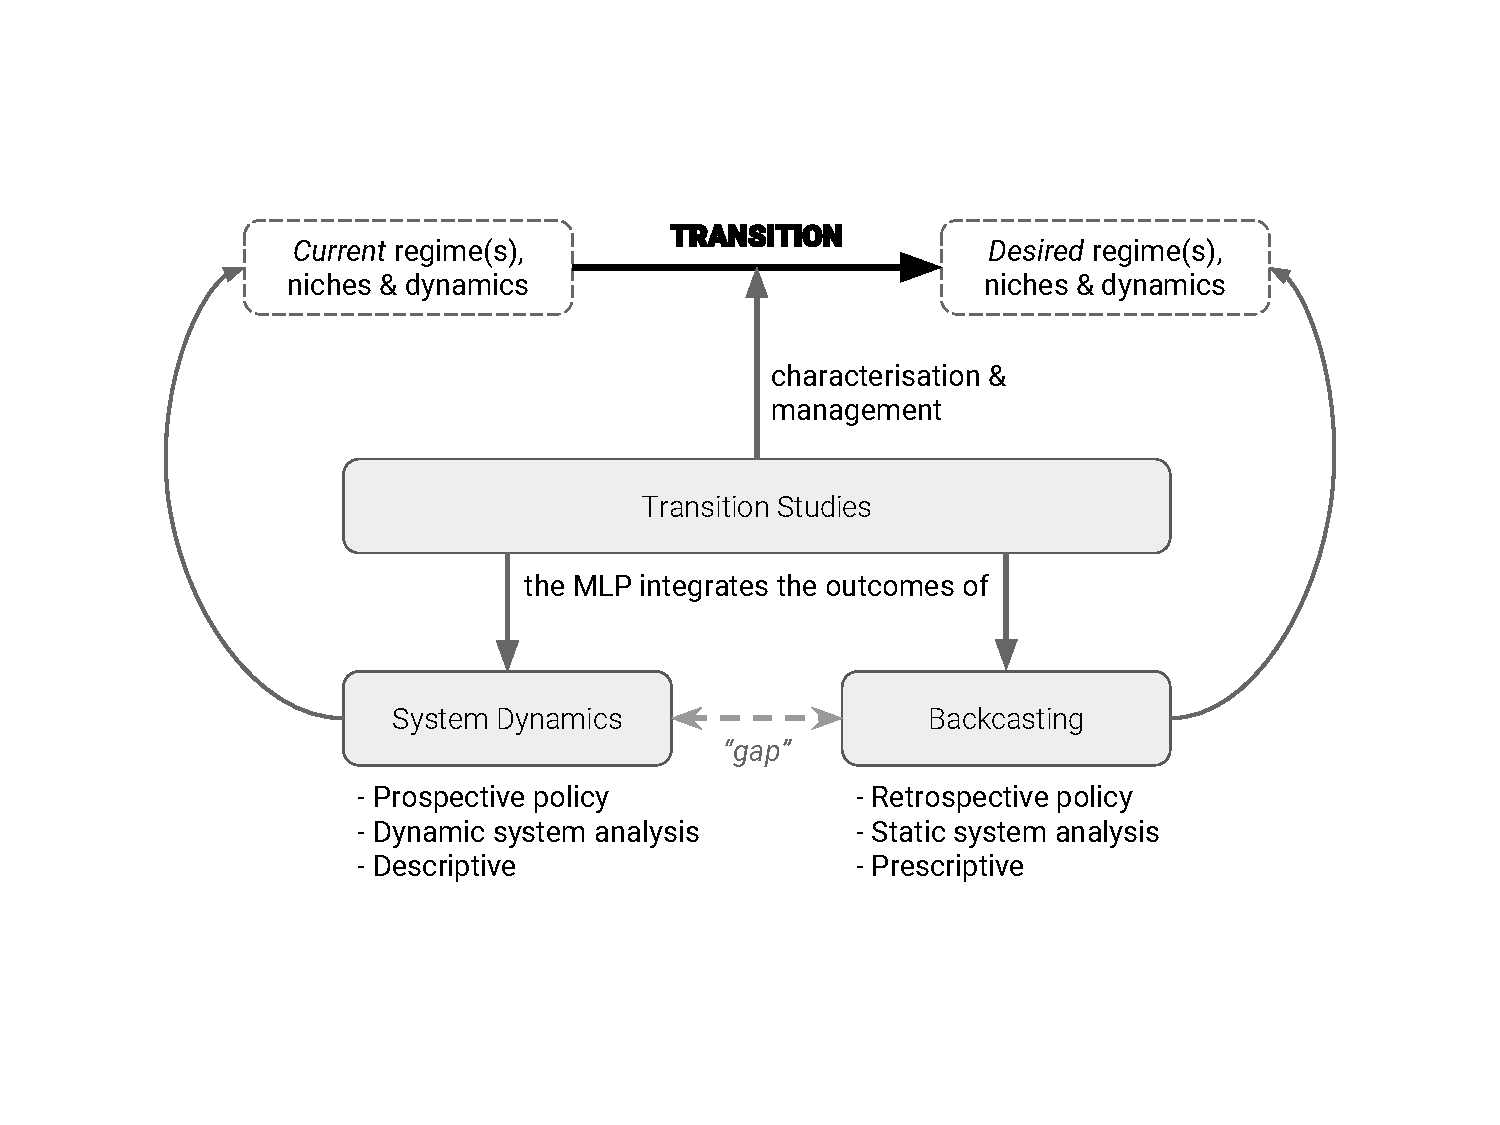
\includegraphics[clip,trim=0 3cm 0 3cm,width=\linewidth]{figures/discussion-methods.pdf}
\caption[Integrative power of transition theory]{Transition theory can bridge the gap between futures studies and forecasting tools, by translating the insights from each into the same language (discourse).}
\label{f:discussion-methodology}
\end{figure}

On one hand, forecasting tools (CLDs and System Dynamics, for example) are commonly used to inform policy makers of the possible development scenarios, but fail to convey normative insights: they are inherently \emph{descriptive} methods. Another weakness of using forecasts as the basis for policy making is that no space is available for radical innovation. This is, predictions based on present system structures cannot take into account structural change or unexpected developments. The policies that emerge from using forecasts are \emph{prospective}. On the other hand, the strength of forecasts and System Dynamics (CLDs) in particular, is the capability to analyse \emph{dynamic}\footnote{Again, the dynamism captured by these tools is constrained to the modelled structure of the system.} behaviours. Dynamics and feedback structures are very important to policy assessment, because they are sources of policy resistance mechanisms, such as rebound effects.

Backcasting and ``desirable'' visions methods are, on the contrary, normative in nature, this is, they are \emph{prescriptive} in their analysis (or discussion) of the systems under scope. However, unless explicitly incorporated in the processes, the perspective of the systems is rather \emph{static}. Even though they are used to convey the desired changes (dynamism over time), they do not account for feedback structures nor for dynamic system behaviour. In the context of sustainable transitions, a final feature of backcasting is appealing as a methodology: the \emph{retrospective} approach to policy design. The fact that backcasting processes start from a desired end-state opens the possibility to include radical innovation or, simply, ``radical'' changes that would be unthinkable from the present system condition.

The use of the MLP in the thesis as a discursive translation tool serves the purpose of overcoming the limitations described above, while benefiting from the strengths of each tool. (1) The focus on co-evolution and dynamism (stability and change) of socio-technical niches, regimes and landscapes fits perfectly the notion of system dynamics captured by CLDs. (2) While not normative per se, the MLP can still accommodate the results of a backcasted pathway to a normative future vision. (3) The context of a ``transition'' embeds desired future visions and pathways and, therefore, policy design can be made retrospectively, allowing broader possibilities to be included and for policies that support radical innovation. Finally, the multidisciplinary approach of the MLP supports an analysis scope broader than that of the formal models of System Dynamics, similarly to backcasting.

As the concluding remark, the aforementioned use of the MLP approach is, as argued, a significant contribution to sustainability research. It could, to some extent, be regarded as a form of \emph{transition management} \parencite{rotmans2001_Moreevolutionthan,kemp2011_TransitionManagementas}, although it differs in some aspects: different emphasis on culture, inclusion of subaltern combined methodologies and, following the transitions governance scheme described by \textcite{kemp2007_Transitionmanagementas}, this thesis is situated only at a strategic management level. However, the approach taken can benefit other sustainability studies in the following situations:
\begin{enumeratealpha}
\item A (participatory) process has delivered a desirable vision and/or pathway to a sustainable future, but there are uncertainties with regards to required structural changes or policy resistance mechanisms.
\item A forecasting study has provided decision makers with a thorough understanding of the current system and its feedback mechanisms but, even at the light of possible scenarios described by the forecast, they are unsure of what normative actions should be taken.
\end{enumeratealpha}
In both cases, a complementary study can be performed and the results can be then harmonised using an MLP approach. This integration framework is, indeed, the most interesting outcome of the thesis.

\section{Further research}
\label{s:discussion:further}
The main line of research that stems from the work in this thesis is the investigation of policy analysis frameworks. This is, researching whether transition theory, and the MLP in particular, can help in the design of policies that fit sustainability better than the current paradigm. In this respect, the scholars from the transitions management field have already made progress, but their approach is a little different. Whereas they focus on niche support and long term goals, this thesis also emphasises the ability of the MLP as an integrative narrative for more ``specific'' assessment tools.

A straightforward extension of the thesis would be to carry out the backcasting process (and the development of the qualitative narrative that serves as the guideline) in a participatory setting. This way, different policy results might be derived or, at the very least, confirmed and validated by stakeholders and general participants. Democracy is, unfortunately, a forgone aspect of sustainability studies. In the case of the thesis, due to time and resources constraints, but in a more general case, due to technocratic views on what science and research is all about. Lengthier study settings, such as PhD research or government officials could undertake this effort.

The usage of Causal Loop Diagrams in combination with other policy design mechanisms is an interesting contribution that deserves further work as well. Most of the literature on System Dynamics and CLDs deals with narrower scopes and bounded systems than what has been studied here. In particular, they are (almost) never used to model ``soft'' issue such as cultural frameworks. Despite the difficulty to quantify these aspects, the argument of this thesis is that CLDs could be used to mentally model these very important issues. They definitely serve the purpose of making mental models explicit, especially when developed in workshops or through Group Model Building techniques.

%The results are contrasted with the literature in \sref{s:discussion:coherency} and, finally,
%\section{Coherency with the literature}
%\label{s:discussion:coherency}
%The thesis is, despite the aforementioned limitations, aligned with the current body of literature on sustainable mobility futures. For example, \textcite{banister2008_sustainablemobilityparadigm} describes four main categories of action that must be pursued to reach the sustainable mobility paradigm he argues for:
\begin{enumerate}
\item Reduce the need for travel through substitution.
\item Encourage modal shift through transport policy measures.
\item Reduce trip lengths through sustainable spatial planning.
\item Encourage higher efficiency in transport through vehicle and fuel technology innovation.
\end{enumerate}
This thesis, on the other side, advocates for very similar results. The backcasted changes are also categorised in four main fronts of action: (1) cultural changes to reduce the overall mobility demand, (2) land-use changes to reduce trip lengths and demand, (3) encouraging modal shift through demand management and intermodal travel and (4) increase vehicle and fuel efficiencies. This similarity is no coincidence. Both \textcite{banister2008_sustainablemobilityparadigm} and this thesis are built on the realisation that the current and historic paradigm of mobility is obsolete from a sustainability point of view and both studies focus on the transformation (or transition) of the system into a new paradigm.



\todoparagraph{In general, the thesis ``outcomes'' are ``biased'', personal and not too generalizable. But! The combination of policy-making tools through the ``discoursive''/``narrative'' power of transition studies is a really interesting result. Even though more work needs to be devoted to this, it clearly suggests that by using the terminology of transition theories, we can bridge the gap between seeminlgy different approaches and tools. This can be very useful in the context of policy-making and (future(s)) sustainability studies, since it promises to deliver a more coherent and integrated result than other approaches.}
\chapter{Conclusion}
\label{c:conclusion}

% Back matter: references and appendices
\backmatter
%\nocite{*} % remove the comment to automatically include all references that are not directly cited in the document

\renewcommand{\UrlFont}{\footnotesize}
\printbibliography

\appendix
%\clearpage
\chapter{IPCC SSP1 storyline summary table}
\label{a:ssp1-summary-table}
%
\tref{t:appendix:ssp1-storyline-summary} corresponds to the summary of the original SSP1 scenario narrative. The original table contained the trends for the rest of the SSP scenarios. Reprinted from Global Environmental Change, \textbf{42}, Brian C. O’Neill, Elmar Kriegler, Kristie L. Ebi, Eric Kemp-Benedict, Keywan Riahi, Dale S. Rothman, Bas J. van Ruijven, Detlef P. van Vuuren, Joern Birkmann, Kasper Kok, Marc
Levy, William Solecki, \textit{The roads ahead: Narratives for shared socioeconomic pathways describing world futures in the 21st century}, 169-180, Copyright (2017), with permission from Elsevier. License number 4111240276671.

{\scriptsize
\begin{longtable}{p{5cm}p{9cm}}
\caption[IPCC's SPP1 storyline summary table.]{IPCC's SPP1 storyline summary table. Adapted from \textcite{oneill2017_roadsaheadNarratives}.}\\
\toprule
SSP element & SSP1 trend \\
\midrule
\endfirsthead
\caption*{(\emph{continued}) IPCC's SPP1 storyline summary table. Adapted from \textcite{oneill2017_roadsaheadNarratives}.}\\
\toprule
SSP element & SSP1 trend \\
\midrule
\endhead
\bottomrule
\endfoot
\bottomrule
\addlinespace
\multicolumn{2}{l}{
\textsuperscript{*}\emph{HIC} stands for \emph{H}igh \emph{I}ncome \emph{C}ountries, \emph{MIC} for \emph{M}edium \emph{I}ncome \emph{C}ountries and \emph{LIC} for \emph{L}ow \emph{I}ncome \emph{C}ountries.}
\endlastfoot
\label{t:appendix:ssp1-storyline-summary}\textbf{Demographics} &  \\
Population growth & Relatively low \\
Fertility rate & Low in currently high- and low-fertility countries; medium in rich OECD countries. \\
Mortality & Low \\
Migration & Medium \\
Urbanization level & High \\
Urbanization type & Well managed \\ \addlinespace
\textbf{Human development} &  \\
Education & High \\
Health investments & High \\
Access to health facilities, water, sanitation & High \\
Gender equality & High \\
Equity & High \\
Social cohesion & High \\
Societal participation & High \\ \addlinespace
\textbf{Economy \& lifestyle} &  \\
Growth (per capita) & High in LICs\textsuperscript{*} and MICs\textsuperscript{*}, medium in HICs\textsuperscript{*} \\
Inequality & Reduced across and within countries \\
International trade & Moderate \\
Globalization & Connected markets, regional production \\
Consumption and diet & Low growth in material consumption, low-meat diets, first in HICs \\
\textbf{Policies \& institutions} &  \\
International cooperation & Effective \\
Environmental policy & Improved management of local and global issues; tighter regulation of pollutants \\
Policy orientation & Toward sustainable development \\
Institutions & Effective at national and international levels \\ \addlinespace
\textbf{Technology} &  \\
Development & Rapid \\
Transfer & Rapid \\
Energy tech. change & Directed away from fossil fuels, toward efficiency and renewables \\
Carbon intensity & Low \\
Energy intensity & Low \\ \addlinespace
\textbf{Environment \& natural resources} &  \\
Fossil constraints & Preferences shift away from fossil fuels \\
Environment & Improving conditions over time \\
Land use & Strong regulations to avoid environmental tradeoffs \\
Agriculture & Improvements in agricultural productivity; rapid diffusion of best practices
\end{longtable}
} %Rajib said not to include this!

\end{document}
